\chapter{न्यूरॉन, क्रिया विभव और तंत्रिका-संधियाँ}\label{ch:b2:neurons-synapses}

घुटने की चपनी के नीचे की कंडरा पर ठोकिए और वह टाँग तीस
मिलीसेकंड बाद झटका मारती है। उस समय में जाँघ में कोई तनाव
भाँपा जा चुका है, कोई संकेत मेरुरज्जु तक मीटर भर चल चुका है, किसी
दूसरी कोशिका तक एक जोड़ पार कर चुका है, मीटर भर वापस चल चुका है और किसी
पेशी को सिकोड़ चुका है --- यानी पूरा चक्कर किसी पलक झपकने से भी तेज़। कोई
\omterm{def:b2:cell-signalling:kinds}{हॉर्मोन} यह नहीं कर सकता था; यह वे कोशिकाएँ करती हैं जो चालन के लिए बनी हैं, और
ऐसा कोई संकेत जो कोई चलता पदार्थ नहीं बल्कि किसी झिल्ली पर फिर-फिर
जनी जाती विद्युत् की कोई तरंग है। यह अध्याय उसी कोशिका और
उसी संकेत के बारे में है: वह वोल्टता जो कोई \omterm{def:b2:neurons-synapses:neuron}{न्यूरॉन} अपनी झिल्ली के आरपार थामे रहता है, वह
आवेग जो वह छोड़ता है और वह आवेग चलता कैसे है, और वह \omterm{def:b2:neurons-synapses:synapse}{तंत्रिका-संधि} जहाँ
वह विद्युत् संकेत किसी रासायनिक में और फिर वापस बदला जाता है।

\section{न्यूरॉन}

\begin{definition}[न्यूरॉन, तंत्रिकाक्ष, तंत्रिका]\label{def:b2:neurons-synapses:neuron}
\index{न्यूरॉन}\index{तंत्रिकाक्ष}\index{द्रुमिका}\index{मायलिन}\index{ग्लिया}
\emph{न्यूरॉन} संकेतन के लिए विशेषीकृत कोई कोशिका है: अपने केंद्रक वाली
एक कोशिका-काया (\emph{सोमा}), संकेत लेती शाखित \emph{द्रुमिकाएँ},
और एक ही \emph{तंत्रिकाक्ष} --- यानी कोई ऐसी केबल जो
माइक्रोमीटर भर से बीस माइक्रोमीटर तक मोटी और मीटर भर तक लंबी है ---
जो उसका निर्गम दूसरी कोशिकाओं पर बने \emph{सिरों} तक ढोता है।
मानव मस्तिष्क में कोई $10^{11}$ न्यूरॉन हैं और हर एक लगभग
हज़ार \omterm{def:b2:neurons-synapses:synapse}{तंत्रिका-संधियाँ} बनाता है। न्यूरॉनों से अधिक \emph{ग्लिया} हैं: वे तारा-कोशिकाएँ
जो उन्हें पोसती तथा उनके लिए बफ़र बनती हैं, वे सूक्ष्म-ग्लिया जो उनकी चौकसी करती हैं, और वे
कोशिकाएँ जो तंत्रिकाक्षों को \emph{मायलिन} में लपेटती हैं --- यानी अपनी ही झिल्ली के
दर्जनों फेरे, जो कोशिकाद्रव से लगभग मुक्त हैं और कोई रोधी ग़िलाफ़ बनाते हैं
जो हर मिलीमीटर भर पर \emph{\omterm{prop:b2:neurons-synapses:myelin}{रैन्वियर की गाँठों}} पर टूटता है।
कोई \emph{तंत्रिका} हज़ारों तंत्रिकाक्षों का एक गट्ठर है, संवेदी तथा प्रेरक,
जो संयोजी ऊतक में साथ चलते हैं। न्यूरॉन वयस्क में विभाजित नहीं
होते (कुछ अपवादों को छोड़कर), और अपनी काया से कटा कोई तंत्रिकाक्ष मर जाता है; कोई
न्यूरॉन ऐसी कोशिका है जिसे जीवन भर चलना है।
\end{definition}

\begin{omfigure}
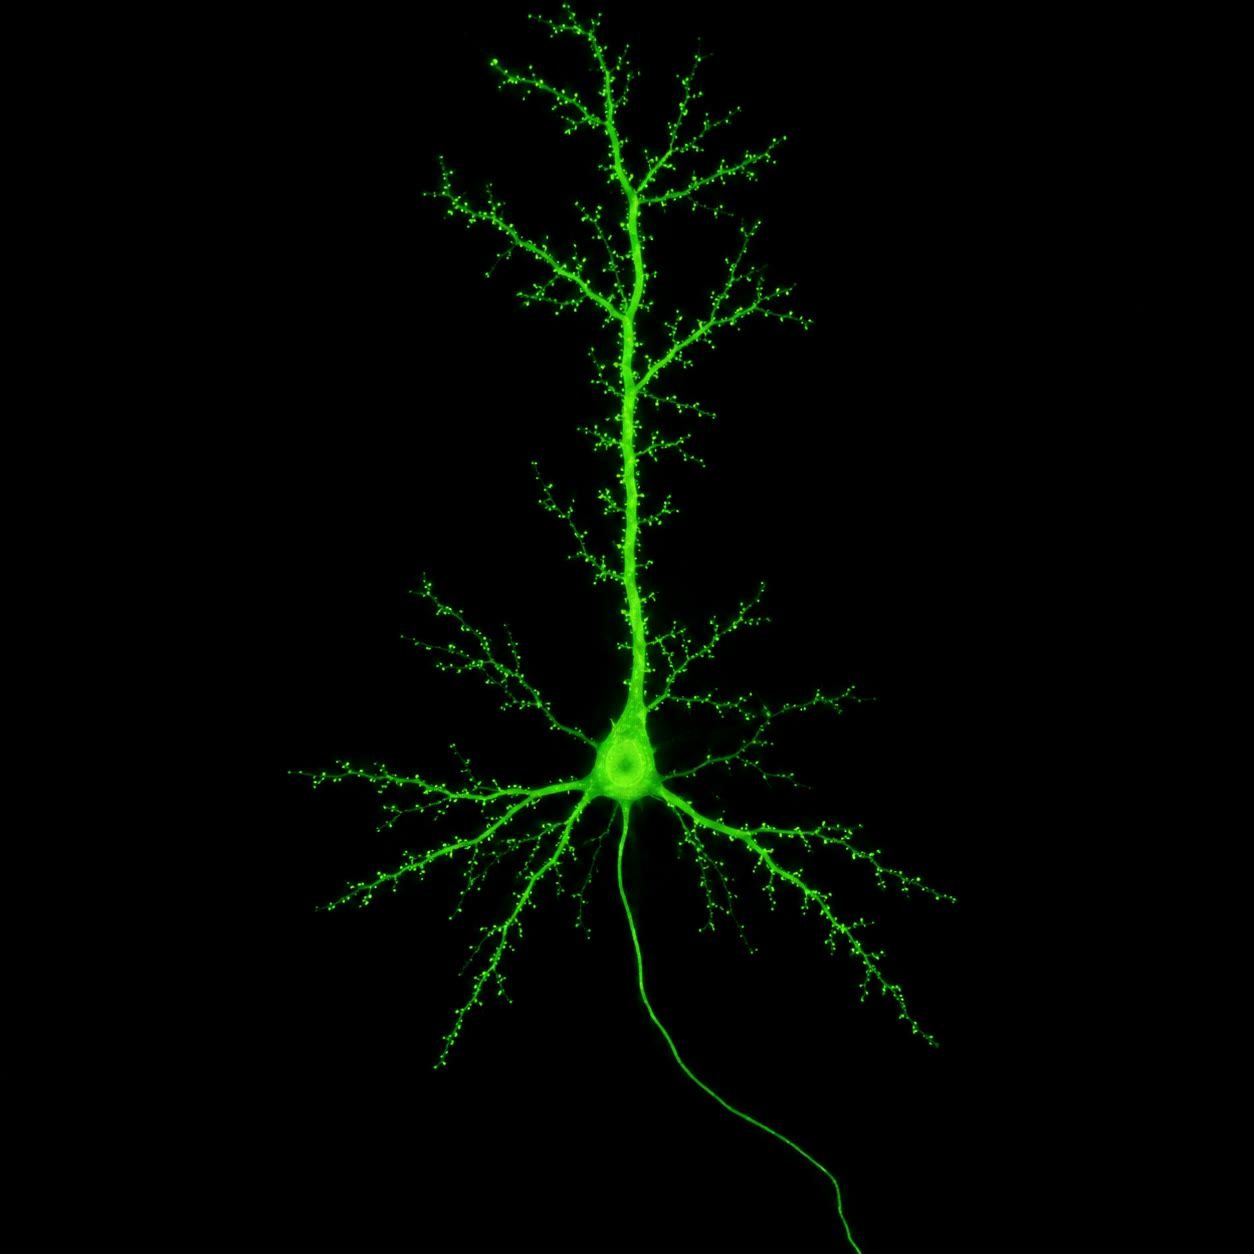
\includegraphics[width=0.4\linewidth]{images/book4/ai/b4-20-neuron-fluorescence.jpg}\hspace{0.05\linewidth}
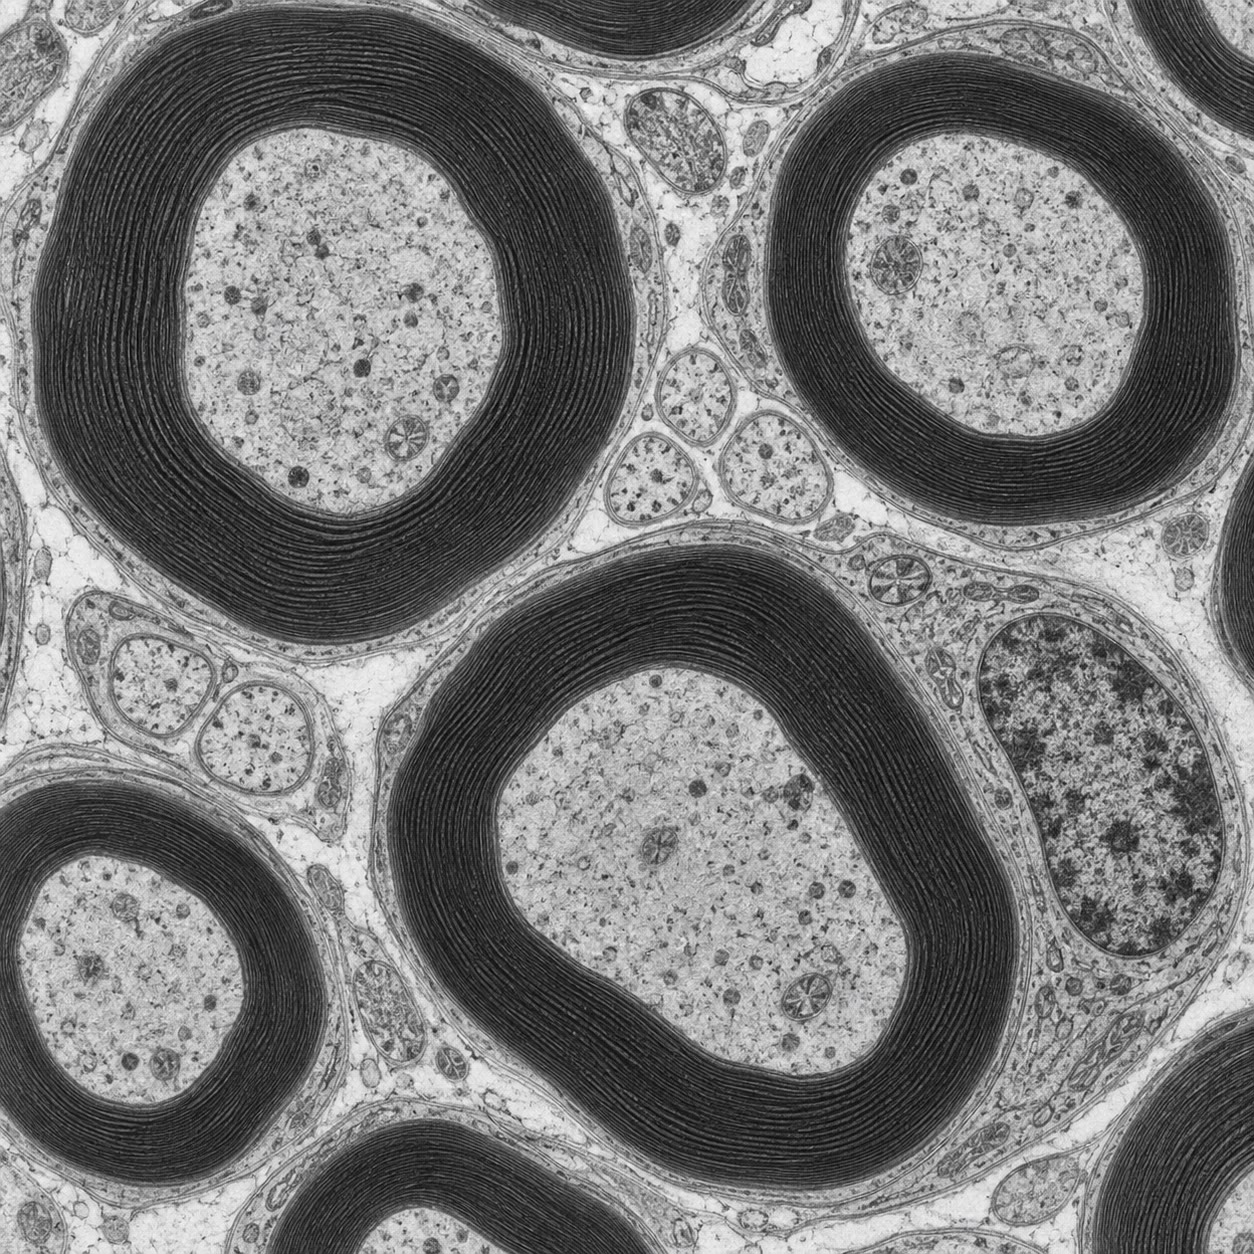
\includegraphics[width=0.4\linewidth]{images/book4/ai/b4-20-myelinated-axons-tem.jpg}

{\small बाएँ: रंजक से भरा कोई पिरामिडी \omterm{def:b2:neurons-synapses:neuron}{न्यूरॉन} --- वह कोशिका-काया,
वे काँटेदार \omterm{def:b2:neurons-synapses:neuron}{द्रुमिकाएँ} जो लेती हैं, और वह पतला \omterm{def:b2:neurons-synapses:neuron}{तंत्रिकाक्ष} जो उस
आधार से निकलता है। दाएँ: इलेक्ट्रॉन सूक्ष्मदर्शी के नीचे अनुप्रस्थ काट में \omterm{def:b2:neurons-synapses:neuron}{तंत्रिकाक्ष},
हर एक अपने \omterm{def:b2:neurons-synapses:neuron}{मायलिन} ग़िलाफ़ के गहरे कुंडल में लिपटा।}
\end{omfigure}

\section{विश्राम विभव}

\begin{theorem}[नर्न्स्ट विभव]\label{thm:b2:neurons-synapses:nernst}
\index{नर्न्स्ट विभव}\index{साम्य विभव}
$z$ आवेश के किसी एक आयन के लिए पारगम्य और $c_{\text{बाहर}}$ तथा
$c_{\text{भीतर}}$ सांद्रताओं को अलग करती कोई झिल्ली उस
\emph{\omterm{thm:b2:neurons-synapses:nernst}{साम्य विभव}} पर बैठ जाती है जिस पर उस आयन पर विद्युत् बल
उसके विसरण को संतुलित करता है:
\[
E = \frac{RT}{zF}\ln\frac{c_{\text{बाहर}}}{c_{\text{भीतर}}} \approx \frac{\qty{61.5}{mV}}{z}\log_{10}\frac{c_{\text{बाहर}}}{c_{\text{भीतर}}} \quad (\qty{37}{\celsius}).
\]
कोई \omterm{def:b2:neurons-synapses:neuron}{न्यूरॉन} बाहर की \qty{5}{mmol/L} के विरुद्ध भीतर \qty{140}{mmol/L}
पोटैशियम थामे रहता है, और बाहर की \qty{145}{mmol/L} के विरुद्ध भीतर
\qty{15}{mmol/L} सोडियम, और ये प्रवणताएँ
सोडियम--पोटैशियम पंप कोशिका की एक तिहाई ATP के दाम पर बनाता है।
इससे $E_{\mathrm K} = 61.5\log_{10}(5/140) = \qty{-89}{mV}$ और
$E_{\mathrm{Na}} = 61.5\log_{10}(145/15) = \qty{+61}{mV}$: यदि वह
झिल्ली केवल पोटैशियम को जाने दे तो वह \qty{-89}{mV} पर बैठती,
और केवल सोडियम को दे तो \qty{+61}{mV} पर।
\end{theorem}
\begin{proof}
साम्य पर उस आयन का विद्युत्-रासायनिक विभव दोनों ओर
वही है: $RT\ln c_{\text{भीतर}} + zFV_{\text{भीतर}} = RT\ln
c_{\text{बाहर}} + zFV_{\text{बाहर}}$, इसलिए $V_{\text{भीतर}} -
V_{\text{बाहर}} = (RT/zF)\ln(c_{\text{बाहर}}/c_{\text{भीतर}})$।
\qty{310}{K} पर, $RT/F = \qty{26.7}{mV}$ और $\ln 10 \times 26.7 =
\qty{61.5}{mV}$। (वर्ष 1 के खंड में बोल्ट्ज़मान
बंटन से निकाला गया; यहाँ फिर से कहा गया।)
\end{proof}

\begin{theorem}[भारित माध्य के रूप में विश्राम विभव]\label{thm:b2:neurons-synapses:chord}
\index{विश्राम विभव}\index{चालकता (झिल्ली)}
यदि वह झिल्ली कई आयन चालित करे, और हर एक की चालकता $g_i$ हो
(यानी वह सहजता जिससे वह उसे गुज़ारती है, जो खुली वाहिकाओं की संख्या से बैठती है),
तो वह स्थिर विभव जिस पर वे धाराएँ कट जाती हैं, यह है:
\[
V = \frac{\sum_i g_i E_i}{\sum_i g_i},
\]
यानी चालकताओं से भारित \omterm{thm:b2:neurons-synapses:nernst}{साम्य विभवों} का कोई माध्य।
विश्राम में किसी \omterm{def:b2:neurons-synapses:neuron}{न्यूरॉन} की झिल्ली सोडियम से लगभग बीस गुना अधिक
पोटैशियम के लिए पारगम्य है, इसलिए $V \approx (20\times(-89) +
61)/21 = \qty{-82}{mV}$; और क्लोराइड तथा छोटे रिसाव
गिन लेने पर \omterm{thm:b2:neurons-synapses:chord}{विश्राम विभव} \qty{-70}{mV} है। वह झिल्ली
$E_{\mathrm K}$ के पास विश्राम करती है क्योंकि पोटैशियम वाहिकाएँ खुली हैं; और जो भी
सोडियम वाहिकाएँ खोले वह उसे $E_{\mathrm{Na}}$ की ओर घसीटता है --- और यही
तंत्रिका-संकेतन का पूरा सिद्धांत है।
\end{theorem}
\begin{proof}
हर आयन कोई धारा $I_i = g_i(V - E_i)$ ढोता है (ओम का नियम, जिसमें
वह चालक बल उस आयन के अपने साम्य से मापा जाता है)। किसी
स्थिर विभव पर कुल धारा शून्य है: $\sum_i g_i(V - E_i) =
0$, जिससे $V\sum g_i = \sum g_iE_i$। (पूरा उपचार, जिसमें
वे पारगम्यताएँ गोल्डमान--हॉजकिन--काट्ज़
समीकरण से घुसती हैं, प्रथम कोटि में वही भारण देता है।)
\end{proof}

\section{क्रिया विभव}

\begin{proposition}[वह आवेग]\label{prop:b2:neurons-synapses:ap}
\index{क्रिया विभव}\index{वोल्टता-द्वारित वाहिका}\index{देहली}\index{अपवर्तक काल}
\omterm{def:b2:neurons-synapses:neuron}{तंत्रिकाक्ष} की झिल्ली \emph{वोल्टता-द्वारित सोडियम वाहिकाएँ} रखती है, जो
विश्राम में बंद हैं और विध्रुवण से खुलती हैं। यदि कोई उद्दीपन उस
विभव को \qty{-70}{mV} से \qty{-55}{mV} के पास की किसी
\emph{देहली} के पार चढ़ा दे, तो उनमें से इतनी खुल जाती हैं कि उतना सोडियम भीतर आए जितना
पोटैशियम का रिसाव काट न सके; वह विभव चढ़ता है, और वाहिकाएँ खुलती हैं,
और किसी मिलीसेकंड के अंश भर में वह झिल्ली
$E_{\mathrm{Na}}$ की ओर बह जाती है --- यानी कोई \emph{धन प्रतिपुष्टि} जो विस्फोटक
तथा सब-या-कुछ-नहीं वाली है। वह \qty{+40}{mV} के पास शिखर पाती है क्योंकि वे सोडियम
वाहिकाएँ खुलने के किसी मिलीसेकंड के भीतर \emph{निष्क्रिय} हो जाती हैं और
क्योंकि धीमी \emph{वोल्टता-द्वारित पोटैशियम वाहिकाएँ} खुलती हैं और
उस विभव को वापस $E_{\mathrm K}$ की ओर चलाती हैं, और पोटैशियम वाहिकाओं के बंद होने से पहले
किसी \emph{अधोक्षेप} तक लाँघ जाती हैं। वह
\emph{\omterm{prop:b2:neurons-synapses:ap}{क्रिया विभव}} लगभग मिलीसेकंड भर चलता है; और एक-दो
मिलीसेकंड और तक वे निष्क्रिय सोडियम वाहिकाएँ फिर नहीं खुल सकतीं
(यानी \emph{\omterm{prop:b2:neurons-synapses:ap}{अपवर्तक काल}}), जो उस दगने की दर को प्रति सेकंड कुछ
सौ तक सीमित करता है और उस आवेग को एक ही ओर चलने पर बाध्य करता है।
चूँकि वह सब-या-कुछ-नहीं वाला है, इसलिए वह आवेग अपने आकार में कोई सूचना नहीं ढोता:
वह \omterm{def:b2:neurons-synapses:neuron}{न्यूरॉन} तीव्रता को अपनी \emph{बारंबारता} में कूटबद्ध करता है। प्रति आवेग कोई
$10^{4}$ सोडियम आयन घुसते हैं और उतने ही पोटैशियम आयन निकलते हैं
--- यानी सांद्रता में कोई नगण्य परिवर्तन, जिसे वह पंप
फ़ुरसत से बहाल कर देता है।
\end{proposition}
\begin{proof}[प्रमाण-सामग्री]
हॉजकिन और हक्सली (1952) ने, विद्रूप के विशाल \omterm{def:b2:neurons-synapses:neuron}{तंत्रिकाक्ष} (आधा
मिलीमीटर मोटा, ताकि उसके भीतर कोई तार पिरोया जा सके) और ऐसे किसी
प्रतिपुष्टि प्रवर्धक से जो उस झिल्ली-विभव को किसी भी चुने गए मान पर थामे रखता था
(यानी \emph{वोल्टता क्लैंप}) जबकि उसे थामने के लिए ज़रूरी धारा
अभिलिखित होती थी, उस धारा को किसी पहले भीतरी घटक में, जो स्नान से सोडियम
हटाने पर मिट जाता था, और किसी बाद के
बाहरी घटक में, जो पोटैशियम ढोता था, अलग किया; हर वोल्टता पर मापा कि हर
चालकता समय के साथ कैसे चढ़ी तथा गिरी; और, हर एक को कुछ समीकरणों से बैठाकर,
\omterm{prop:b2:neurons-synapses:ap}{क्रिया विभव} का आकार, देहली, गति तथा \omterm{prop:b2:neurons-synapses:ap}{अपवर्तक काल}
केवल उन दो चालकताओं से गिन लिया।
हर भविष्यवाणी टिकी। वे वाहिकाएँ स्वयं पच्चीस वर्ष बाद देखी गईं,
एक-एक करके, पैच क्लैंप से;
टेट्रोडोटॉक्सिन (पफ़रमछली का विष) सोडियम वाहिका रोकता है
और वह आवेग मिटा देता है, और टेट्राएथिलअमोनियम पोटैशियम
वाहिका रोकता है और उसे लंबा कर देता है।
\end{proof}

\begin{omfigure}
\begin{tikzpicture}
\begin{axis}[
  width=0.9\linewidth, height=6.4cm,
  axis x line=bottom, axis y line=left,
  xmin=0, xmax=4, ymin=-100, ymax=60,
  xlabel={समय (ms)}, ylabel={झिल्ली-विभव (mV)},
  xlabel style={font=\small, at={(axis description cs:0.5,-0.1)}, anchor=north},
  ylabel style={font=\small},
  tick label style={font=\small}, xtick={0,1,2,3,4}, ytick={-90,-70,-55,0,40},
  legend style={font=\scriptsize, at={(0.97,0.95)}, anchor=north east, draw=none},
  clip=false,
]
\addplot[very thick, omDef] coordinates {(0,-70) (0.4,-70) (0.5,-64) (0.6,-55) (0.7,-30) (0.8,10) (0.9,35) (1.0,40) (1.1,30) (1.2,10) (1.35,-20) (1.5,-50) (1.7,-75) (1.9,-85) (2.2,-82) (2.6,-76) (3.2,-71) (4,-70)};
\addlegendentry{झिल्ली-विभव}
\addplot[thick, omThm, dashed] coordinates {(0,0) (0.5,0) (0.6,5) (0.7,20) (0.8,35) (0.9,30) (1.0,20) (1.1,8) (1.2,3) (1.4,0) (4,0)};
\addlegendentry{$g_{\mathrm{Na}}$ (सापेक्ष)}
\addplot[thick, omProp, dashed] coordinates {(0,0) (0.6,0) (0.8,2) (1.0,8) (1.2,16) (1.4,20) (1.7,17) (2.0,10) (2.4,4) (3.0,1) (4,0)};
\addlegendentry{$g_{\mathrm K}$ (सापेक्ष)}
\draw[dashed, gray] (axis cs:0,-55) -- (axis cs:4,-55); \node[font=\scriptsize, anchor=south east] at (axis cs:4,-55) {देहली};
\draw[dashed, gray] (axis cs:0,-89) -- (axis cs:4,-89); \node[font=\scriptsize, anchor=south east] at (axis cs:3.7,-89) {$E_{\mathrm K}$};
\draw[<->, gray] (axis cs:1.0,50) -- (axis cs:2.5,50); \node[font=\scriptsize, anchor=south, gray] at (axis cs:1.75,50) {अपवर्तक};
\end{axis}
\end{tikzpicture}

{\small कोई \omterm{prop:b2:neurons-synapses:ap}{क्रिया विभव}। देहली के पार सोडियम-चालकता
(लाल) विस्फोटक ढंग से चढ़ती है और उस विभव को $E_{\mathrm{Na}}$ की ओर
चलाती है; वह निष्क्रिय हो जाती है ज्यों ही पोटैशियम-चालकता
(नारंगी) चढ़ती है और उस झिल्ली को किसी अधोक्षेप के साथ $E_{\mathrm K}$ की ओर
लौटाती है। देहली-रेखा से नीचे कुछ नहीं होता।}
\end{omfigure}

\section{चालन}

\begin{theorem}[वह केबल और उसका लंबाई-नियतांक]\label{thm:b2:neurons-synapses:cable}
\index{लंबाई-नियतांक}\index{केबल समीकरण}\index{चालन वेग}
कोई \omterm{def:b2:neurons-synapses:neuron}{तंत्रिकाक्ष} कोई रिसती केबल है: किसी बिंदु पर डाली गई धारा
कोशिकाद्रव्य के साथ बहती है (प्रति इकाई लंबाई प्रतिरोध $r_i$) और उस
झिल्ली से होकर रिसती है (प्रतिरोध $r_m$ गुणा इकाई लंबाई)। कोई स्थिर
विध्रुवण $V_0$, $x = 0$ पर, उस \omterm{def:b2:neurons-synapses:neuron}{तंत्रिकाक्ष} के साथ इस तरह क्षीण होता है:
\[
V(x) = V_0\,e^{-x/\lambda}, \qquad \lambda = \sqrt{\frac{r_m}{r_i}} = \sqrt{\frac{R_m\,d}{4R_i}},
\]
जिसमें $d$ वह व्यास है और $R_m$, $R_i$ झिल्ली तथा
कोशिकाद्रव्य के विशिष्ट प्रतिरोध। \emph{लंबाई-नियतांक}
$\lambda$ वह दूरी है जिस पर कोई निष्क्रिय संकेत गिरकर
एक तिहाई रह जाता है: किसी \qty{1}{\micro m} \omterm{def:b2:neurons-synapses:neuron}{तंत्रिकाक्ष} के लिए लगभग \qty{0.5}{mm}, जो
उस व्यास के वर्गमूल के साथ बढ़ता है। कोई \omterm{prop:b2:neurons-synapses:ap}{क्रिया विभव} इसलिए
संचरित होता है कि उसके अग्र भाग पर वह विध्रुवण, आगे लगभग $\lambda$ भर
निष्क्रिय रूप से फैलकर, झिल्ली के अगले टुकड़े को
देहली तक ले आता है, जो उसे पूरे आकार में फिर जन देता है; और वह जितना आगे तक
पहुँचे, वह तरंग उतनी तेज़, इसलिए वह \omterm{thm:b2:neurons-synapses:cable}{चालन वेग} भी
मोटे तौर पर $\sqrt{d}$ की तरह बढ़ता है --- किसी पतले
बिना-मायलिन तंतु में \qty{1}{m/s} से विद्रूप के विशाल \omterm{def:b2:neurons-synapses:neuron}{तंत्रिकाक्ष} में \qty{20}{m/s} तक।
\end{theorem}
\begin{proof}
मान लीजिए $i(x)$ अक्षीय धारा है और $V(x)$ झिल्ली का
विध्रुवण। तंत्रिकाद्रव्य के साथ ओम का नियम देता है $\mathrm{d}V/
\mathrm{d}x = -r_i\,i$; और आवेश का संरक्षण, झिल्ली से होकर उस रिसाव समेत,
देता है $\mathrm{d}i/\mathrm{d}x = -V/r_m$। मिलाने पर,
$\mathrm{d}^{2}V/\mathrm{d}x^{2} = V/(r_m r_i)$, जिसका क्षीण होता
हल $V_0 e^{-x/\lambda}$ है, $\lambda^{2} = r_m/r_i$ के साथ। किसी
बेलन के लिए, $r_m = R_m/(\pi d)$ और $r_i = 4R_i/(\pi d^{2})$, इसलिए
$\lambda^{2} = R_m d/4R_i$। $R_m = \qty{1}{\ohm.m^2}$, $R_i =
\qty{1}{\ohm.m}$ और $d = \qty{1}{\micro m}$ के साथ: $\lambda = \sqrt{10^{-6}
/4} = \qty{0.5}{mm}$।
\end{proof}

\begin{proposition}[मायलिन और लंघन चालन]\label{prop:b2:neurons-synapses:myelin}
\index{लंघन चालन}\index{रैन्वियर की गाँठ}
\omterm{def:b2:neurons-synapses:neuron}{मायलिन} $r_m$ को झिल्ली-फेरों की संख्या से गुणा करता है और
झिल्ली की धारिता को उसी गुणक से बाँट देता है, ताकि उस
ग़िलाफ़ के नीचे लगभग कोई धारा न रिसे और उस विभव को बदलने के लिए थोड़ा ही आवेश चाहिए:
वह विध्रुवण मिलीमीटर भर के किसी अंतर-गाँठ के साथ थोड़ी हानि के साथ
निष्क्रिय रूप से फैल जाता है, और वह \omterm{prop:b2:neurons-synapses:ap}{क्रिया विभव}
केवल उन गाँठों पर फिर जना जाता है, जहाँ वे सोडियम वाहिकाएँ
सघन हैं। इस तरह वह आवेग गाँठ से गाँठ \emph{कूदता} है
(यानी \emph{\omterm{prop:b2:neurons-synapses:myelin}{लंघन चालन}}), किसी \qty{20}{\micro m} तंतु में
\qty{100}{m/s} पर --- यानी वह गति जिसके लिए किसी बिना-मायलिन \omterm{def:b2:neurons-synapses:neuron}{तंत्रिकाक्ष} को
सेंटीमीटरों मोटा होना पड़ता --- और उपापचयी लागत के किसी अंश पर,
क्योंकि सोडियम केवल गाँठों पर घुसता है। \omterm{def:b2:neurons-synapses:neuron}{मायलिन}
कशेरुकियों का वह आविष्कार है जिसने किसी छोटी देह में कोई बड़ा, तेज़ तंत्रिका तंत्र
संभव बनाया; और बहु-काठिन्य में वह ग़िलाफ़
टुकड़ा-टुकड़ा नष्ट हो जाता है, वह लंबाई-नियतांक ढह जाता है, और वे
आवेग चूक जाते हैं।
\end{proposition}

\begin{omfigure}
\begin{tikzpicture}[every node/.style={font=\scriptsize}, >=stealth]
  % unmyelinated
  \begin{scope}
    \draw[thick, fill=omDef!10] (0,0) rectangle (11,0.5);
    \foreach \x in {0.5,1.0,...,10.5} \draw[omThm, ->] (\x,0.25) -- (\x,0.9);
    \node[anchor=east] at (-0.2,0.25) {बिना मायलिन};
    \node[anchor=west] at (11.2,0.25) {\qty{1}{m/s}};
    \node[above] at (5.5,1.0) {वह आवेग हर बिंदु पर फिर जना जाता है};
  \end{scope}
  % myelinated
  \begin{scope}[yshift=-2.4cm]
    \draw[thick, fill=omDef!10] (0,0) rectangle (11,0.5);
    \foreach \x in {0.3,2.5,4.7,6.9,9.1} \fill[omExo!60] (\x,-0.15) rectangle (\x+1.9,0.65);
    \foreach \x in {2.35,4.55,6.75,8.95} \draw[omThm, ->] (\x,0.25) -- (\x,0.9);
    \foreach \x in {2.35,4.55,6.75} \draw[->, thick, omThm, dashed] (\x+0.1,1.1) .. controls (\x+1.1,1.6) .. (\x+2.1,1.1);
    \node[anchor=east] at (-0.2,0.25) {मायलिन वाला};
    \node[anchor=west] at (11.2,0.25) {\qty{100}{m/s}};
    \node[below] at (1.25,-0.2) {मायलिन अंतर-गाँठ};
    \node[below] at (4.55,-0.2) {रैन्वियर की गाँठ};
    \node[above] at (5.5,1.6) {केवल गाँठों पर फिर जना: लंघन};
  \end{scope}
\end{tikzpicture}

{\small \omterm{def:b2:neurons-synapses:neuron}{मायलिन} के साथ और बिना चालन। किसी नंगे \omterm{def:b2:neurons-synapses:neuron}{तंत्रिकाक्ष} में वह
आवेग सारे रास्ते फिर जना जाता है; जबकि \omterm{def:b2:neurons-synapses:neuron}{मायलिन} के नीचे वह संकेत हर अंतर-गाँठ के साथ
निष्क्रिय रूप से फैलता है और गाँठों पर फिर जना जाता है, और
वह आवेग सौ गुना तेज़ चलता है।}
\end{omfigure}

\section{तंत्रिका-संधि}

\begin{definition}[रासायनिक और विद्युत् तंत्रिका-संधियाँ]\label{def:b2:neurons-synapses:synapse}
\index{तंत्रिका-संधि}\index{तंत्रिकासंचारी}\index{पश्चसंधि विभव}
किसी \emph{तंत्रिका-संधि} पर किसी \omterm{def:b2:neurons-synapses:neuron}{न्यूरॉन} का सिरा किसी लक्ष्य से मिलता है --- किसी दूसरे
\omterm{def:b2:neurons-synapses:neuron}{न्यूरॉन} से, किसी पेशी-तंतु से, किसी ग्रंथि-कोशिका से। किसी \emph{विद्युत्}
संधि में गैप संधियाँ दोनों कोशिकाएँ जोड़ देती हैं और धारा सीधे गुज़रती है
--- यानी तेज़, दोतरफ़ा, बिना प्रवर्धन के, और वहाँ काम में ली जाती है जहाँ गति तथा
समकालिकता मायने रखती हैं (पलायन-प्रतिवर्त, \omterm{def:b2:heart:anatomy}{हृदय})। किसी \emph{रासायनिक}
संधि में वे कोशिकाएँ \qty{20}{nm} की किसी दरार से अलग हैं और वह
संकेत कोई अणु है। उस सिरे पर पहुँचता कोई \omterm{prop:b2:neurons-synapses:ap}{क्रिया विभव}
वोल्टता-द्वारित कैल्सियम वाहिकाएँ खोलता है; कैल्सियम घुसती है और, किसी
मिलीसेकंड के अंश भर के भीतर, \emph{तंत्रिकासंचारी} की पुटिकाओं को
उस झिल्ली से जुड़ने और उस दरार में उड़ेलने पर लगा देती है; वह संचारी
माइक्रोसेकंडों में आरपार विसरित होता है और पश्चसंधि झिल्ली पर ग्राहियों से
बँधता है --- या तो ऐसे आयन-वाहिकाओं से जिन्हें वह खोलता है
(\emph{आयनोट्रॉपिक}, तेज़) या G-प्रोटीन-युग्मित ग्राहियों से
(\emph{मेटाबोट्रॉपिक}, धीमे, \cref{ch:b2:cell-signalling}); और उससे
बनी धारा पश्चसंधि विभव को कुछ
मिलिवोल्ट खिसका देती है, ऊपर (कोई \emph{उत्तेजक पश्चसंधि विभव},
सोडियम गुज़ारती वाहिकाओं से) या नीचे (कोई \emph{संदमक}, क्लोराइड या
पोटैशियम गुज़ारती वाहिकाओं से); और वह संचारी
मिलीसेकंडों के भीतर किसी एंजाइम या किसी वाहक से हटा दिया जाता है। वह
देरी आधा मिलीसेकंड है; और वह दाम एकतरफ़ा संचरण,
प्रवर्धन, संदमन तथा परिवर्तनीयता ख़रीद लेता है --- यानी वह सब जो किसी
तंत्रिका तंत्र को मात्र चालन से आगे चाहिए।
\end{definition}

\begin{omfigure}
\begin{tikzpicture}[every node/.style={font=\scriptsize}, >=stealth]
  % presynaptic terminal
  \draw[thick, fill=omDef!10] (0,0) .. controls (0,2.6) and (3.6,2.6) .. (3.6,0.2) -- (3.6,-0.2) .. controls (3.6,-2.6) and (0,-2.6) .. (0,0);
  \draw[very thick, omDef] (-2.2,0) -- (0.1,0); \node[omDef, above] at (-1.1,0.05) {तंत्रिकाक्ष};
  \foreach \p in {(2.0,1.0),(2.6,0.5),(2.7,-0.4),(2.1,-1.0),(1.6,0.2)} \draw[thick, fill=omProp!40] \p circle (0.25);
  \draw[thick, fill=omProp!40] (3.3,0.1) arc (90:-90:0.25) -- cycle;
  \foreach \p in {(3.75,0.2),(3.85,-0.1),(3.7,-0.35),(3.9,0.4)} \fill[omProp] \p circle (0.05);
  \fill[omThm] (3.45,1.3) circle (0.06); \node[omThm, anchor=east] at (3.35,1.45) {Ca$^{2+}$ घुसती है};
  \draw[->, omThm] (3.9,1.5) -- (3.55,1.35);
  % cleft
  \node[align=center, anchor=north] at (3.85,-2.75) {दरार\\\qty{20}{nm}};
  \draw[gray] (3.85,-2.7) -- (3.85,-1.2);
  % postsynaptic
  \draw[thick, fill=omExo!15] (4.1,-2.6) rectangle (8.2,2.6);
  \foreach \y in {0.9,0.3,-0.3,-0.9} \draw[thick, fill=omDef!40] (4.05,\y-0.15) rectangle (4.45,\y+0.15);
  \node[anchor=west, align=left] at (4.6,0.3) {ग्राही: वाहिकाएँ\\खुलती हैं, आयन बहते हैं,\\पश्चसंधि\\विभव};
  \node[anchor=west, align=left] at (4.6,-1.7) {संचारी एंजाइम या\\वाहक से\\हटाया गया};
  \node[anchor=west] at (4.6,2.2) {पश्चसंधि कोशिका};
  % labels
  \node[align=center, anchor=north] at (1.8,-2.75) {संचारी की\\पुटिकाएँ};
  \node[anchor=south] at (1.8,2.75) {पूर्वसंधि सिरा};
\end{tikzpicture}

{\small कोई रासायनिक \omterm{def:b2:neurons-synapses:synapse}{तंत्रिका-संधि}। वह आवेग कैल्सियम भीतर लेता है, पुटिकाएँ
जुड़ती हैं और उस दरार में संचारी छोड़ती हैं, उस लक्ष्य पर ग्राही
वाहिकाएँ खोलते हैं, और वह संचारी मिलीसेकंडों के भीतर
साफ़ कर दिया जाता है।}
\end{omfigure}

\begin{theorem}[अंशीय मोचन]\label{thm:b2:neurons-synapses:quantal}
\index{अंशीय मोचन}\index{लघु विभव}
संचारी पुड़ियों में छोड़ा जाता है --- यानी \emph{अंश}, हर एक में एक पुटिका
--- और किसी एक आवेग से छोड़ी गई संख्या $k$ कोई यादृच्छिक
चर है। यदि वह सिरा $n$ मोचन-स्थल रखे और हर एक
प्रायिकता $p$ से छोड़े, और $p$ छोटी हो, तो $k$ लगभग पॉइसों है,
माध्य $m = np$ के साथ:
\[
P(k) = \frac{m^{k}e^{-m}}{k!}, \qquad P(0) = e^{-m}, \qquad
m = \ln\frac{\text{प्रयासों की संख्या}}{\text{विफलताओं की संख्या}}.
\]
इसलिए माध्य अंश-मात्रा $m$ उन आवेगों के अंश से पढ़ी जा सकती है
जो कुछ भी नहीं छोड़ते, और उसे एक अंश के आकार से बँटी
माध्य अनुक्रिया से जाँचा जा सकता है। किसी
\omterm{prop:b2:neurons-synapses:integration}{तंत्रिका-पेशी संधि} पर $m$ कुछ सौ है --- वहाँ संचरण कभी नहीं
चूकता; जबकि किसी केंद्रीय \omterm{def:b2:neurons-synapses:synapse}{तंत्रिका-संधि} पर वह अक्सर एक के पास है, और वह संधि
आवेगों के किसी अंश पर ही संचरित करती है।
\end{theorem}
\begin{proof}
$n$ स्वतंत्र स्थलों के साथ, हर एक प्रायिकता $p$ से छोड़ता, $k$
द्विपद है; और बड़े $n$ तथा छोटी $p$ के लिए, $np = m$ नियत रखते हुए, वह
द्विपद पॉइसों नियम की ओर जाता है (गणित की शृंखला, वर्ष 2)।
$P(0) = e^{-m}$ उन विफलताओं से $m$ देता है। काट्ज़ की जाँच यह है कि
वही $m$, उस पॉइसों सूत्र में डालकर, एक, दो तथा तीन अंशों की अनुक्रियाओं के
देखे गए अंशों की भविष्यवाणी करता है।
\end{proof}
\begin{proof}[प्रमाण-सामग्री]
फ़ैट और काट्ज़ (1952) ने विश्राम में किसी मेंढक-पेशी-तंतु से
लगभग \qty{0.5}{mV} के छोटे स्वतःस्फूर्त विध्रुवण अभिलिखित किए, सब
एक ही आकार के, यादृच्छिक अंतरालों पर --- यानी वे \emph{लघु अंत्य-पट्ट
विभव}, जिनमें से हर एक किसी एक पुटिका का प्रभाव है। उस स्नान में कैल्सियम
घटाने से तंत्रिका-उद्दीपन की अनुक्रिया तब तक घटी जब तक वह
उस लघु आकार के 0, 1, 2 या 3 गुणजों के बीच उतार-चढ़ाव न करने लगी;
और उन गुणजों की बारंबारताएँ उस $m$ के साथ पॉइसों नियम पर चलीं जो
उन विफलताओं से गिना गया था। इस तरह डेल कास्तिलो और काट्ज़ ने दिखाया
कि मोचन अंशीय है, कि कैल्सियम मोचन की प्रायिकता नियंत्रित करती है
न कि किसी अंश का आकार, और इलेक्ट्रॉन सूक्ष्मदर्शिकी ने
वे पुटिकाएँ दिखाईं जो वे अंश हैं।
\end{proof}

\begin{proposition}[समाकलन: किसी निर्णय के रूप में न्यूरॉन]\label{prop:b2:neurons-synapses:integration}
\index{संकलन}\index{तंत्रिकाक्ष-टीला}\index{तंत्रिका-पेशी संधि}
कोई केंद्रीय \omterm{def:b2:neurons-synapses:neuron}{न्यूरॉन} अपनी \omterm{def:b2:neurons-synapses:neuron}{द्रुमिकाओं} तथा सोमा पर हज़ारों \omterm{def:b2:neurons-synapses:synapse}{तंत्रिका-संधियाँ} पाता है,
उत्तेजक तथा संदमक। हर \omterm{def:b2:neurons-synapses:synapse}{पश्चसंधि विभव}
छोटा है और निष्क्रिय रूप से क्षीण होता है, स्थान में उस केबल के लंबाई-नियतांक के साथ
और समय में उस झिल्ली के काल-नियतांक (कुछ मिलीसेकंड) के साथ;
वे जुड़ते हैं --- साथ पहुँचते निवेशों का \emph{स्थानिक संकलन},
जल्दी-जल्दी पहुँचते निवेशों का \emph{कालिक संकलन} --- और वह योग
\emph{तंत्रिकाक्ष-टीले} पर पढ़ा जाता है, जहाँ
वे सोडियम वाहिकाएँ सबसे सघन हैं और वह देहली सबसे नीची। यदि वह
योग देहली पार कर ले तो वह \omterm{def:b2:neurons-synapses:neuron}{तंत्रिकाक्ष} दगता है, ऐसी दर पर जो उस अधिकता के साथ
चढ़ती है; और संदमक निवेश घटाते हैं, तथा उस टीले के पास कोई संदमक \omterm{def:b2:neurons-synapses:synapse}{तंत्रिका-संधि}
किसी दूर के उत्तेजक पर वीटो लगा सकती है। वह
\omterm{prop:b2:neurons-synapses:integration}{तंत्रिका-पेशी संधि} वह अपवाद है जो उस नियम को दिखाता है: कोई एक
प्रेरक सिरा, जो ऐसिटिलकोलीन के सैकड़ों अंश ऐसे ग्राहियों पर छोड़ता है
जो स्वयं वाहिकाएँ भी हैं, \qty{50}{mV} का कोई अंत्य-पट्ट विभव
देता है, यानी देहली से कहीं ऊपर --- प्रेरक तंत्रिका में हर आवेग
कोई पेशी-क्रिया विभव पैदा करता है
(\cref{ch:b2:muscle-movement})। क्यूरारे, जो उस ग्राही को रोकता है,
लकवा मार देता है; और तंत्रिका-गैसें, जो ऐसिटिलकोलीन हटाने वाले उस एंजाइम को
रोकती हैं, उलटी अधिकता से लकवा मारती हैं।
\end{proposition}

\begin{example}[संचारी और दवाएँ]\label{ex:b2:neurons-synapses:transmitters}
\omterm{prop:b2:neurons-synapses:integration}{तंत्रिका-पेशी संधि} पर तथा स्वायत्त तंत्र में
ऐसिटिलकोलीन; ग्लूटामेट, यानी मस्तिष्क का मुख्य उत्तेजक संचारी,
और GABA, यानी मुख्य संदमक; एकल-ऐमीन नॉरऐड्रिनैलिन,
डोपामीन तथा सेरोटोनिन, जो कुछ हज़ार कोशिकाओं से पूरे-पूरे परिपथ
साधते हैं; और दर्जनों पेप्टाइड। मन पर काम करती लगभग हर दवा
किसी \omterm{def:b2:neurons-synapses:synapse}{तंत्रिका-संधि} पर काम करती है: बेंज़ोडाइऐज़ेपीन GABA की
वाहिका मज़बूत करते हैं, अवसादरोधी सेरोटोनिन का वाहक रोकते हैं, कोकीन
डोपामीन का रोकती है, अफ़ीमज किसी पेप्टाइड की नक़ल करते हैं, निकोटीन
एक ग्राही पर ऐसिटिलकोलीन की नक़ल करती है और ऐट्रोपीन दूसरे पर उसे रोकती है,
और बोटुलिनम विष वे प्रोटीन काट देता है जो उस पुटिका को जोड़ते हैं। वह \omterm{def:b2:neurons-synapses:synapse}{तंत्रिका-संधि}
वही है जहाँ \cref{ch:b2:cell-signalling} का रसायन और
इस अध्याय की विद्युत् मिलते हैं, और जहाँ कोई तंत्रिका तंत्र सीखता है:
जो \omterm{def:b2:neurons-synapses:synapse}{तंत्रिका-संधियाँ} काम में ली जाएँ वे मज़बूत होती हैं, और वह मज़बूती (वर्ष 3
का खंड) स्मृति है।
\end{example}

\section{अभ्यास}

\begin{exercise}[$\star$]\label{exo:b2:neurons-synapses:1}
किसी \omterm{def:b2:neurons-synapses:neuron}{न्यूरॉन} के भागों और हर एक का कार्य बताइए, और कहिए कि
\omterm{def:b2:neurons-synapses:neuron}{मायलिन} किसका बना है और वह क्या करता है।
\end{exercise}

\begin{exercise}[$\star$]\label{exo:b2:neurons-synapses:2}
किसी \omterm{prop:b2:neurons-synapses:ap}{क्रिया विभव} की अवस्थाओं और हर एक का कारण बनने वाली वाहिका-घटनाओं का
वर्णन कीजिए। वह सब-या-कुछ-नहीं वाला क्यों है, और वह पीछे की ओर क्यों नहीं
चलता?
\end{exercise}

\begin{exercise}[$\star$]\label{exo:b2:neurons-synapses:3}
किसी रासायनिक \omterm{def:b2:neurons-synapses:synapse}{तंत्रिका-संधि} पर उस आवेग के पहुँचने से उस संचारी के हटाए जाने तक
संचरण के चरण गिनाइए।
\end{exercise}

\begin{exercise}[$\star$]\label{exo:b2:neurons-synapses:4}
विद्युत् तथा रासायनिक \omterm{def:b2:neurons-synapses:synapse}{तंत्रिका-संधियों} की तुलना गति, दिशा,
प्रवर्धन तथा संदमन की संभावना में कीजिए।
\end{exercise}

\begin{exercise}[$\star\star$]\label{exo:b2:neurons-synapses:5}
\qty{37}{\celsius} पर पोटैशियम (140 भीतर, 5 बाहर), सोडियम (15 भीतर, 145 बाहर),
क्लोराइड (10 भीतर, 110 बाहर)
तथा कैल्सियम (\qty{1e-4}{} भीतर, 2 बाहर, \unit{mmol/L} में) के लिए \omterm{thm:b2:neurons-synapses:nernst}{नर्न्स्ट विभव} निकालिए। झिल्ली के
\qty{-70}{mV} पर होने पर हर आयन किस ओर बहता है?
\end{exercise}

\begin{exercise}[$\star\star$]\label{exo:b2:neurons-synapses:6}
$E_{\mathrm K} = \qty{-89}{mV}$ तथा $E_{\mathrm{Na}} =
\qty{+61}{mV}$ के साथ, झिल्ली-विभव निकालिए जब $g_{\mathrm K} :
g_{\mathrm{Na}} = 20 : 1$ (विश्राम), $1 : 20$ (उस आवेग का शिखर)
तथा $50 : 1$ (वह अधोक्षेप) हो। हर दशा को समझाइए।
\end{exercise}

\begin{exercise}[$\star\star$]\label{exo:b2:neurons-synapses:7}
बिना-मायलिन \omterm{def:b2:neurons-synapses:neuron}{तंत्रिकाक्षों} में \omterm{thm:b2:neurons-synapses:cable}{चालन वेग} $\sqrt d$ की तरह चलता है, और
\qty{1}{\micro m} पर \qty{1}{m/s} है। किसी \qty{0.5}{mm} विद्रूप-तंत्रिकाक्ष का
वेग निकालिए। कोई \omterm{def:b2:neurons-synapses:neuron}{मायलिन} वाला \qty{20}{\micro m} तंतु
\qty{100}{m/s} पर चालन करता है: उससे मेल खाने के लिए किसी बिना-मायलिन \omterm{def:b2:neurons-synapses:neuron}{तंत्रिकाक्ष} को
कितना मोटा होना पड़ता? हर तंतु में कोई आवेग मेरुरज्जु से
पैर की उँगली तक (\qty{1}{m}) कितना समय लेता है?
\end{exercise}

\begin{exercise}[$\star\star$]\label{exo:b2:neurons-synapses:8}
किसी \omterm{def:b2:neurons-synapses:synapse}{तंत्रिका-संधि} की नीची कैल्सियम में 200 उद्दीपनाओं में से 74 कोई
अनुक्रिया नहीं देतीं। माध्य अंश-मात्रा और एक, दो तथा तीन अंशों की
अनुक्रियाओं के भविष्यवाणित अंश निकालिए। एक अंश
\qty{0.5}{mV} का है: कौन-सी माध्य अनुक्रिया अपेक्षित है?
\end{exercise}

\begin{exercise}[$\star\star$]\label{exo:b2:neurons-synapses:9}
किसी \omterm{def:b2:neurons-synapses:neuron}{न्यूरॉन} का \omterm{prop:b2:neurons-synapses:ap}{अपवर्तक काल} \qty{2}{ms} है। उसकी अधिकतम
दगने की दर क्या है? कोई संवेदी \omterm{def:b2:neurons-synapses:neuron}{न्यूरॉन} किसी हल्के स्पर्श के लिए प्रति सेकंड 20
आवेग और किसी कड़े के लिए 200 दगता है: क्या कूटबद्ध है, और किससे?
\end{exercise}

\begin{exercise}[$\star\star\star$]\label{exo:b2:neurons-synapses:10}
$R_m = \qty{1}{\ohm.m^2}$, $R_i =
\qty{1}{\ohm.m}$ तथा 1, 10 और \qty{500}{\micro m} व्यासों के लिए
लंबाई-नियतांक निकालिए। \omterm{def:b2:neurons-synapses:neuron}{मायलिन} $R_m$ को 200 से गुणा करता है:
\qty{10}{\micro m} के लिए फिर से निकालिए। समझाइए कि \qty{1}{mm} का कोई
अंतर-गाँठ क्यों चलता है और \qty{3}{mm} का कोई बिना-मायलिन टुकड़ा उसे क्यों रोक देता है।
\end{exercise}

\begin{exercise}[$\star\star\star$]\label{exo:b2:neurons-synapses:11}
इनके \omterm{prop:b2:neurons-synapses:ap}{क्रिया विभव} पर और \omterm{prop:b2:neurons-synapses:integration}{तंत्रिका-पेशी संधि} पर संचरण पर
प्रभाव की भविष्यवाणी कीजिए: टेट्रोडोटॉक्सिन; टेट्राएथिलअमोनियम; बिना
कैल्सियम का कोई स्नान; क्यूरारे; कोई ऐसिटिलकोलिनएस्टरेज़ संदमक;
बोटुलिनम विष।
\end{exercise}

\begin{exercise}[$\star\star\star$]\label{exo:b2:neurons-synapses:12}
``कोई रासायनिक \omterm{def:b2:neurons-synapses:synapse}{तंत्रिका-संधि} आधा मिलीसेकंड लेती है और कोई तंत्रिका तंत्र
ख़रीद लेती है।'' उस देरी से क्या मिलता है --- एकतरफ़ा संचरण,
प्रवर्धन, संदमन, सुनम्यता --- इस पर विचार कीजिए, और यह कि देह
उसके बजाय विद्युत् \omterm{def:b2:neurons-synapses:synapse}{तंत्रिका-संधियाँ} कहाँ काम में लेती है।
\end{exercise}

\section{समस्या: घुटने का झटका समयबद्ध}

\begin{problem}[{सप्तांत समस्या --- तनाव-प्रतिवर्त कंडरा पर ठोकने से उस
झटके तक पीछा किया गया, और उस न्यूरॉन का विश्राम विभव
गिना, उस आवेग का चालन उस चाप की दोनों भुजाओं पर समयबद्ध, उस
तंत्रिका-संधि की अंश-मात्रा मापी, और पूरी विलंबता का लेखा दिया,
और अंत उस विश्राम विभव, उन चालन-कालों, उस
अंश-मात्रा तथा उस प्रतिवर्त-विलंबता पर}]
\label{pb:b2:neurons-synapses:1}
\qty{37}{\celsius} पर आँकड़े: पोटैशियम 140 भीतर, 4 बाहर; सोडियम 12 भीतर,
145 बाहर (\unit{mmol/L}); विश्राम में $g_{\mathrm K} : g_{\mathrm{Na}} = 25 : 1$।
संवेदी तथा प्रेरक \omterm{def:b2:neurons-synapses:neuron}{तंत्रिकाक्ष}: \qty{15}{\micro m}, \omterm{def:b2:neurons-synapses:neuron}{मायलिन} वाले,
\qty{90}{m/s}, हर ओर \qty{0.9}{m}। संधि-देरी \qty{0.6}{ms};
पेशी का अपने ही \omterm{prop:b2:neurons-synapses:ap}{क्रिया विभव} के बाद सक्रियण \qty{5}{ms}।
नीची कैल्सियम में केंद्रीय \omterm{def:b2:neurons-synapses:synapse}{तंत्रिका-संधि}: 300 प्रयास, 111 विफलताएँ। अंश
\qty{0.4}{mV}; देहली विश्राम से \qty{15}{mV} ऊपर। $R_m =
\qty{1}{\ohm.m^2}$, $R_i = \qty{1}{\ohm.m}$; \omterm{def:b2:neurons-synapses:neuron}{मायलिन} $R_m$ को
250 से गुणा करता है।

\medskip
\noindent\textbf{भाग I --- विश्राम करता \omterm{def:b2:neurons-synapses:neuron}{न्यूरॉन}।}
\begin{enumerate}
  \item $E_{\mathrm K}$ और $E_{\mathrm{Na}}$ निकालिए।
  \item उस चालकता-अनुपात से \omterm{thm:b2:neurons-synapses:chord}{विश्राम विभव} निकालिए।
  \item बाह्यकोशिकीय पोटैशियम चढ़कर \qty{8}{mmol/L} हो जाती है (जैसे
        कड़े व्यायाम के बाद)। $E_{\mathrm K}$ तथा वह
        \omterm{thm:b2:neurons-synapses:chord}{विश्राम विभव} फिर से निकालिए, और कहिए कि यह उत्तेजनीयता का क्या करता है।
  \item वह पंप रुक जाता है। समझाइए कि घंटों भर उन प्रवणताओं तथा उस
        विभव का क्या होता है, और वह कोशिका क्यों फूलती है।
  \item यदि झिल्ली की धारिता \qty{0.01}{F/m^2} हो और वह विभव
        \qty{100}{mV} झूले, तो प्रति आवेग प्रति मिलीमीटर किसी
        \qty{15}{\micro m} \omterm{def:b2:neurons-synapses:neuron}{तंत्रिकाक्ष} में कितने सोडियम आयन घुसते हैं?
        ($Q = CV$; एक आयन \qty{1.6e-19}{C} ढोता है।)
  \item वह भीतरी सोडियम-सांद्रता को किस अंश से
        बदलता है (प्रति मिलीमीटर \omterm{def:b2:neurons-synapses:neuron}{तंत्रिकाक्ष} का आयतन)?
  \item वह पंप प्रति ATP तीन सोडियम आयन बाहर भेजता है। प्रति मिलीमीटर \omterm{def:b2:neurons-synapses:neuron}{तंत्रिकाक्ष}
        एक आवेग उलटने में कितनी ATP लगती है?
\end{enumerate}

\medskip
\noindent\textbf{भाग II --- चालन।}
\begin{enumerate}[resume]
  \item संवेदी आवेग को मेरुरज्जु तक और प्रेरक आवेग को उस पेशी तक
        पहुँचने का काल निकालिए।
  \item किसी नंगे \qty{15}{\micro m} \omterm{def:b2:neurons-synapses:neuron}{तंत्रिकाक्ष} का और \omterm{def:b2:neurons-synapses:neuron}{मायलिन} के नीचे उसी
        \omterm{def:b2:neurons-synapses:neuron}{तंत्रिकाक्ष} का लंबाई-नियतांक निकालिए।
  \item कोई अंतर-गाँठ \qty{1.5}{mm} है। उस गाँठीय विध्रुवण का कौन-सा
        अंश \omterm{def:b2:neurons-synapses:neuron}{मायलिन} के साथ तथा बिना निष्क्रिय रूप से अगली गाँठ तक
        पहुँचता है? कौन-सी स्थिति अगली गाँठ को देहली तक
        (\qty{100}{mV} के किसी आवेग से \qty{15}{mV}) ला सकती है?
  \item बिना \omterm{def:b2:neurons-synapses:neuron}{मायलिन}, वही \omterm{def:b2:neurons-synapses:neuron}{तंत्रिकाक्ष} $\sqrt{15}$
        m/s पर चालन करता। वह पूरा चक्कर निकालिए और टिप्पणी कीजिए।
  \item \qty{4}{mm} का कोई टुकड़ा अपना \omterm{def:b2:neurons-synapses:neuron}{मायलिन} खो देता है। उसे पार करते
        संकेत का अंश निकालिए और कहिए कि वह प्रतिवर्त
        बचता है या नहीं।
  \item वह \omterm{prop:b2:neurons-synapses:ap}{अपवर्तक काल} उस आवेग को संवेदी \omterm{def:b2:neurons-synapses:neuron}{तंत्रिकाक्ष} पर केवल एक ही
        दिशा में चलने पर क्यों बाध्य करता है?
\end{enumerate}

\medskip
\noindent\textbf{भाग III --- वह \omterm{def:b2:neurons-synapses:synapse}{तंत्रिका-संधि}।}
\begin{enumerate}[resume]
  \item उन विफलताओं से माध्य अंश-मात्रा $m$ निकालिए।
  \item 1, 2 तथा 3 अंशों की अनुक्रियाओं के भविष्यवाणित अंश, और उन 300
        प्रयासों में अपेक्षित संख्याएँ निकालिए।
  \item माध्य \omterm{def:b2:neurons-synapses:synapse}{पश्चसंधि विभव} निकालिए।
  \item सामान्य कैल्सियम में उसी \omterm{def:b2:neurons-synapses:synapse}{तंत्रिका-संधि} की $m = 60$ है। किसी
        विफलता की प्रायिकता, और माध्य अनुक्रिया क्या है? क्या कोई एक
        ऐसी संधि उस प्रेरक \omterm{def:b2:neurons-synapses:neuron}{न्यूरॉन} को दगा देती है?
  \item उस प्रेरक \omterm{def:b2:neurons-synapses:neuron}{न्यूरॉन} को एक साथ सक्रिय ऐसी \num{20} संवेदी \omterm{def:b2:neurons-synapses:synapse}{तंत्रिका-संधियाँ}
        मिलती हैं। समझाइए कि वे कैसे जुड़ती हैं और देहली तक
        पहुँचा जाता है या नहीं।
  \item उसी \omterm{def:b2:neurons-synapses:neuron}{न्यूरॉन} पर कोई संदमक \omterm{def:b2:neurons-synapses:synapse}{तंत्रिका-संधि} क्लोराइड
        वाहिकाएँ खोलती है ($E_{\mathrm{Cl}} = \qty{-70}{mV}$, यानी वह \omterm{thm:b2:neurons-synapses:chord}{विश्राम
        विभव})। समझाइए कि वह उस कोशिका को अति-ध्रुवित किए बिना उस उत्तेजक
        अनुक्रिया को कैसे घटा सकती है।
\end{enumerate}

\medskip
\noindent\textbf{भाग IV --- पूरा प्रतिवर्त।}
\begin{enumerate}[resume]
  \item जोड़िए: संवेदी चालन, संधि-देरी, प्रेरक चालन,
        तंत्रिका-पेशी देरी (\qty{0.6}{ms}), पेशी-सक्रियण। मापे गए
        \qty{30}{ms} से तुलना कीजिए।
  \item मापी गई विलंबता का बाक़ी भाग कहाँ से आता है?
  \item उस प्रतिवर्त में एक ही \omterm{def:b2:neurons-synapses:synapse}{तंत्रिका-संधि} है (एकसंधि)। समझाइए कि कोई
        प्रत्याहरण प्रतिवर्त, जिसमें उस रज्जु में दो या तीन \omterm{def:b2:neurons-synapses:synapse}{तंत्रिका-संधियाँ} हों,
        धीमा पर अधिक लचीला क्यों है।
  \item परिधीय बिना-मायलिन वाली किसी रोगिणी में वही ठोकर
        \qty{60}{ms} देर से कोई प्रतिवर्त देती है। उसकी तंत्रिकाओं में \omterm{thm:b2:neurons-synapses:cable}{चालन
        वेग} आँकिए।
  \item टेट्रोडोटॉक्सिन की कोई ख़ुराक आधी सोडियम वाहिकाएँ रोक देती है।
        उस देहली, उस आवेग तथा उस प्रतिवर्त पर प्रभाव की
        भविष्यवाणी कीजिए।
  \item परिणाम बताइए: वह \omterm{thm:b2:neurons-synapses:chord}{विश्राम विभव}, वे संवेदी तथा
        प्रेरक चालन-काल, वह अंश-मात्रा $m$, और वह
        गिनी गई प्रतिवर्त-विलंबता।
\end{enumerate}
\end{problem}
